\documentclass[journal]{IEEEtran}
\usepackage[spanish,es-tabla]{babel}
\usepackage[utf8]{inputenc}
\usepackage[T1]{fontenc}
\usepackage{amsmath,amssymb,booktabs,array,cite,url,graphicx}
\usepackage{algorithm,algorithmic}
\usepackage{microtype}
\floatname{algorithm}{Algoritmo}
\renewcommand{\algorithmicrequire}{\textbf{Entrada:}}
\renewcommand{\algorithmicensure}{\textbf{Salida:}}
\addto\captionsspanish{\renewcommand{\abstractname}{Abstract}}
\newcommand{\RPD}{\mathrm{RPD}}
\hyphenation{me-ta-heu-rís-ti-cas me-mé-ti-co ge-né-ti-co}
\begin{document}
\title{Comparación de algoritmos genéticos, meméticos y Ant Colony System para minimizar el makespan en el PFSP}
\author{Sebastián~Deschamps, Brandon~Martínez y Luis~Viluñir\\[0.2em]
\normalsize Facultad de Ingeniería, Universidad Católica de la Santísima Concepción\\
\normalsize Algoritmos Metaheurísticos Inspirados en la Naturaleza}
\markboth{}{Deschamps \MakeLowercase{\textit{et al.}}: Comparación de AG, AM y ACS para el PFSP}
\maketitle

\begin{abstract}
This study compares a Genetic Algorithm (GA), a Memetic Algorithm (MA), and an Ant Colony System (ACS) for makespan minimization in the Permutation Flow Shop Scheduling Problem. The algorithms use a common permutation representation, the same makespan evaluator, and explicit random seeds to ensure reproducibility. The evaluation considered three Taillard instances of sizes $20\times5$, $50\times10$, and $100\times10$, using three seeds and 600 iterations per configuration. On the small instance, GA and MA obtained similar average results, and one MA run reached the reference value. On the medium instance, MA achieved the best average solution quality, although it showed greater variation across seeds. On the large instance, GA obtained the lowest relative percentage deviation and CPU time. ACS required the longest execution times and did not outperform the evolutionary methods on the evaluated instances. The results show that performance depends on instance size and that no single algorithm dominates all the studied cases.
\end{abstract}
\begin{IEEEkeywords}
Permutation flow shop, makespan, genetic algorithm, memetic algorithm, ant colony system, Taillard benchmarks.
\end{IEEEkeywords}

\section{Introducción}
\IEEEPARstart{L}{a} programación de trabajos en líneas de producción busca coordinar recursos limitados y reducir el tiempo necesario para completar una carga de trabajo. En el problema del taller de flujo de permutación, o \textit{Permutation Flow Shop Scheduling Problem} (PFSP), todos los trabajos recorren las mismas máquinas y conservan una secuencia común. El objetivo considerado es minimizar el \textit{makespan}, tiempo de finalización del último trabajo. La elección de esa secuencia afecta las esperas entre operaciones incluso cuando los tiempos de procesamiento individuales permanecen constantes.

El espacio de soluciones contiene $n!$ permutaciones para $n$ trabajos. Este crecimiento motiva el uso de procedimientos aproximados que exploren soluciones sin enumerarlas exhaustivamente. Los conjuntos de Taillard permiten estudiar estos procedimientos sobre instancias reproducibles de diferentes dimensiones~\cite{Taillard1993}. Entre los antecedentes clásicos, la heurística NEH construye secuencias mediante inserciones sucesivas~\cite{Nawaz1983}, mientras que Reeves estudia un algoritmo genético para minimizar el makespan en el flow shop de permutación~\cite{Reeves1995}.

Los algoritmos meméticos combinan evolución poblacional y refinamiento individual mediante búsqueda local~\cite{Krasnogor2005}. Por su parte, Ant Colony System (ACS), propuesto por Dorigo y Gambardella para el problema del vendedor viajero, utiliza información heurística y feromonas compartidas para construir soluciones~\cite{Dorigo1997}. Su transferencia al PFSP exige sustituir las distancias por información de procesamiento y evaluar secuencias abiertas mediante el makespan. Las transiciones entre trabajos no representan costos aditivos independientes.

Este trabajo integra AG, AM y ACS en un sistema modular con representación y evaluación comunes. Su objetivo es comparar calidad final, variabilidad, consumo de CPU y convergencia bajo configuraciones explícitas. El aporte metodológico es la adaptación de ACS al PFSP y la unificación de los tres métodos para su evaluación sobre instancias comunes. La experimentación permite estudiar cómo se manifiestan exploración e intensificación en las implementaciones concretas, sin atribuir sus resultados a todas las variantes posibles de cada familia.

\section{Descripción del problema y marco teórico}
\label{sec:problema}
\subsection{Modelo y evaluación común}
Sean $n$ trabajos y $m$ máquinas ordenadas en serie. Cada trabajo visita las máquinas $1,\ldots,m$, sin interrupciones; cada máquina procesa como máximo un trabajo a la vez. Todos están disponibles en el instante cero. Los tiempos $p_{j,k}>0$ son deterministas, sin tiempos de preparación adicionales, bloqueo ni restricciones de espera nula. Una solución es una permutación $\pi=(\pi_1,\ldots,\pi_n)$, idéntica en todas las máquinas.

La finalización del trabajo situado en la posición $i$ sobre la máquina $k$ satisface
\begin{equation}
C(i,k)=\max\{C(i-1,k),C(i,k-1)\}+p_{\pi_i,k},
\label{eq:recurrencia}
\end{equation}
con $C(0,k)=C(i,0)=0$. El problema consiste en
\begin{equation}
\min_{\pi\in\mathcal{S}_n} C_{\max}(\pi),\qquad C_{\max}(\pi)=C(n,m).
\end{equation}
La implementación almacena una matriz de tiempos de forma $n\times m$ e índices internos desde cero. El evaluador compartido construye la matriz de finalización en $O(nm)$ tiempo y espacio; los archivos de salida numeran los trabajos desde uno.

Como ejemplo, para $A=(2,3)$ y $B=(4,1)$, la secuencia $(A,B)$ produce finalizaciones $(2,5)$ y $(6,7)$, con makespan 7. El orden $(B,A)$ produce $(4,5)$ y $(6,9)$, con makespan 9. Ambos órdenes son factibles, pero difieren en la coordinación entre máquinas.

\subsection{Métrica de calidad}
La desviación porcentual relativa permite comparar brechas respecto de una referencia propia de cada instancia:
\begin{equation}
\RPD(\pi)=100\,\frac{C_{\max}(\pi)-C_{\mathrm{ref}}}{C_{\mathrm{ref}}}.
\label{eq:rpd}
\end{equation}
Un valor menor indica mayor calidad; cero significa alcanzar la referencia. Se utilizan 1278, 2991 y 5770 para ta001, ta041 y ta071, respectivamente. Estas referencias proceden del conjunto de soluciones óptimas o mejores conocidas de Gmys, versión 2021~\cite{Gmys2021}. Se conserva esa versión fija para reproducir el cálculo del RPD.

\section{Metodología y diseño de los algoritmos}
\label{sec:metodo}
\subsection{Algoritmo genético}
El AG inicia una población de permutaciones aleatorias. Selecciona cada padre mediante torneo entre dos individuos distintos y conserva al de menor makespan. El cruce OX copia un segmento delimitado por dos posiciones y completa los espacios restantes siguiendo el orden circular del otro padre, omitiendo trabajos ya presentes. Así se preserva la factibilidad sin reparación posterior.

El cruce se aplica con probabilidad $p_c$ por pareja. Cada descendiente incorporado se muta con probabilidad $p_m$, extrayendo un trabajo y reinsertándolo en otra posición. El reemplazo es generacional y conserva una copia del mejor individuo. Este elitismo evita perder la mejor calidad alcanzada, aunque no garantiza mantener diversidad. No se añaden filtros de duplicados ni reinicios poblacionales.

\subsection{Algoritmo memético}
El AM comparte inicialización, selección, cruce, mutación y elitismo con el AG. Cada $K$ generaciones, según el parámetro de frecuencia recibido por línea de comandos, aplica búsqueda local al mejor individuo de la población recién evaluada. Recorre posiciones de origen y destino en orden ascendente, acepta la primera inserción que reduce estrictamente el makespan y reinicia el recorrido desde la solución mejorada. La solución refinada reemplaza al individuo, por lo que puede transmitir su estructura a generaciones posteriores.

Cada aplicación evalúa como máximo $10n$ vecinos, además de evaluar inicialmente la solución recibida. También termina si completa un recorrido sin mejora. El límite permite controlar el costo, pero puede interrumpir la exploración antes de certificar un óptimo local. Como cada vecino se evalúa en $O(nm)$, la búsqueda acotada requiere a lo sumo $O(n^2m)$ por aplicación. El orden determinista favorece examinar primero ciertas posiciones cuando se agota el presupuesto.

\subsection{Adaptación de ACS al PFSP}
En ACS, cada hormiga artificial arma una secuencia de trabajos. Elige el primero y luego agrega trabajos que todavía no ha utilizado, hasta completar la lista. Para representar la elección inicial se agrega un punto ficticio $s$, que no corresponde a un trabajo real.

Las decisiones se apoyan en dos valores: la feromona y la información heurística. La feromona $\tau_{ij}$ es un número que cambia durante la búsqueda y sirve para recordar qué elecciones formaron parte de buenas soluciones. En este caso, se refiere a colocar el trabajo $j$ inmediatamente después del trabajo $i$. La información heurística $\eta_{ij}$ se calcula con los tiempos de procesamiento y sirve como orientación inicial.

La información se guarda por separado para cada orden de trabajos. Esto se debe a que cambiar el orden puede cambiar las esperas entre máquinas y el makespan, como ocurrió en el ejemplo de los trabajos $A$ y $B$. Por eso, el algoritmo no supone que lo aprendido al programar $A$ y luego $B$ también sirve para programar $B$ y luego $A$. Las tablas de feromona y heurística tienen $(n+1)$ filas y $n$ columnas; la fila adicional permite guardar la información para elegir el primer trabajo.

Para calcular la heurística se compara el tiempo del trabajo $j$ en una máquina con el de $i$ en la siguiente. Se suman las diferencias positivas y se ignoran las negativas. Esa suma se llama $d_{ij}$. Para elegir el primer trabajo se usa $d_{sj}$, que suma sus tiempos en las primeras $m-1$ máquinas:
\begin{align}
d_{ij}&=\sum_{k=1}^{m-1}\max\{0,p_{j,k}-p_{i,k+1}\},\\
d_{sj}&=\sum_{k=1}^{m-1}p_{j,k},\qquad
\eta_{ij}=\frac{1}{1+d_{ij}}.\label{eq:heuristica-inicio}
\end{align}
Para elegir el primer trabajo todavía no existe un trabajo anterior. Por eso, cuando $i=s$, se utiliza $d_{sj}$, definido en la ecuación~\eqref{eq:heuristica-inicio}, y se calcula $\eta_{sj}=1/(1+d_{sj})$. Después de elegir el primer trabajo, se utiliza $d_{ij}$ para evaluar los siguientes.

La regla favorece los pares con una suma menor, porque reciben un valor mayor de $\eta_{ij}$. Se utiliza como una aproximación para orientar la elección según posibles esperas. No calcula la espera exacta, ya que esta también depende de los trabajos programados antes. Para saber qué tan buena es una secuencia completa, se calcula su makespan mediante~\eqref{eq:recurrencia}.

Todas las feromonas parten con el mismo valor, $\tau_0=1/[nC_{\max}(\pi_{\mathrm{SPT}})]$. Para obtenerlo se ordenan los trabajos de menor a mayor suma de tiempos de procesamiento, regla llamada SPT, y se calcula el makespan de esa secuencia. SPT se utiliza únicamente para fijar este valor inicial.

Al elegir el siguiente trabajo, la hormiga combina feromona y heurística en un peso $w_{ij}$. El parámetro $\beta$ controla la influencia de la heurística. Si $U$ es el conjunto de trabajos que faltan por programar, se calcula
\begin{equation}
w_{ij}=\tau_{ij}\eta_{ij}^{\beta},\qquad
P(j\mid i,U)=\frac{w_{ij}}{\sum_{u\in U}w_{iu}}.
\end{equation}
La segunda fórmula convierte los pesos en probabilidades: divide el peso de cada opción por la suma de todos ellos. Con probabilidad $q_0$, la hormiga elige directamente el trabajo de mayor peso. En otro caso, realiza un sorteo usando esas probabilidades. Así puede aprovechar las opciones mejor valoradas y también probar otras. Si hay empate en el mayor peso, se elige el trabajo de menor índice.

Después de cada elección se modifica la feromona del paso utilizado. Esta es la actualización local:
\begin{equation}
\tau_{ij}\leftarrow(1-\alpha)\tau_{ij}+\alpha\tau_0.
\label{eq:local}
\end{equation}
La fórmula acerca la feromona a su valor inicial. Si había aumentado por resultados anteriores, ahora disminuye, dando más oportunidad a otras opciones. Las hormigas construyen sus secuencias una después de otra y usan la misma tabla, por lo que cada una encuentra los cambios realizados por las anteriores.

Cuando todas terminan, se calcula el makespan de cada secuencia y se escoge la mejor de esa iteración, llamada $\pi^{\mathrm{it}}$. Solo los pasos que aparecen en ella reciben la actualización global:
\begin{equation}
\tau_{ij}\leftarrow(1-\alpha)\tau_{ij}+\frac{\alpha}{C_{\max}(\pi^{\mathrm{it}})}.
\label{eq:global}
\end{equation}
El aporte depende de $1/C_{\max}$: una secuencia con menor makespan aporta más feromona. También se actualiza el paso desde $s$ al primer trabajo. Los demás pasos no cambian en esta fase. El parámetro $\alpha$ controla cuánto influye el nuevo valor y se usa en ambas actualizaciones.

Por último, se guarda la mejor secuencia encontrada durante toda la ejecución. Esta es la que se entrega como resultado, aunque para actualizar las feromonas se use la mejor de cada iteración. El Algoritmo~\ref{alg:acs} resume el procedimiento; $H$ indica la cantidad de hormigas y $T$ la cantidad de iteraciones.

\begin{algorithm}[t]
\caption{ACS adaptado al PFSP}
\label{alg:acs}
\footnotesize
\begin{algorithmic}[1]
\REQUIRE Tiempos $P$, semilla, $H,T,\alpha,\beta,q_0$.
\ENSURE Mejor secuencia histórica $\pi^*$ y su makespan.
\STATE Inicializar generador, $\eta$, $\tau_0$ y matriz $\tau$.
\STATE $C^*\leftarrow+\infty$.
\FOR{$t=1,\ldots,T$}
  \FOR{$h=1,\ldots,H$}
    \STATE Construir $\pi^h$ desde $s$ sin repetir trabajos.
    \STATE Aplicar~\eqref{eq:local} después de cada elección.
  \ENDFOR
  \STATE Evaluar todas las secuencias mediante~\eqref{eq:recurrencia}.
  \STATE $\pi^{\mathrm{it}}\leftarrow\arg\min_h C_{\max}(\pi^h)$.
  \STATE Actualizar sus aristas mediante~\eqref{eq:global}.
  \IF{$C_{\max}(\pi^{\mathrm{it}})<C^*$}
    \STATE $\pi^*\leftarrow\pi^{\mathrm{it}}$; $C^*\leftarrow C_{\max}(\pi^{\mathrm{it}})$.
  \ENDIF
  \STATE Registrar resultado de iteración, mejor histórico y CPU.
\ENDFOR
\end{algorithmic}
\end{algorithm}

\subsection{Implementación y reproducibilidad}
Los ejecutables \texttt{ag.py}, \texttt{am.py} y \texttt{acs.py} reciben instancia, semilla, parámetros y destino por línea de comandos. Comparten operadores y escritura de CSV en \texttt{operadores.py}. Cada corrida utiliza un generador NumPy inicializado explícitamente. Los registros guardan configuración, secuencias, makespans, RPD y CPU por iteración. Los parámetros que no corresponden al algoritmo ejecutado quedan vacíos en el formato común.

El lector interpreta la cabecera y la matriz de tiempos del formato Taillard, transpone las filas de máquinas a una matriz trabajo--máquina y comprueba dimensiones, tiempos positivos y referencia positiva. Los operadores evolutivos preservan permutaciones; ACS excluye los trabajos ya programados. El mejor histórico se actualiza únicamente ante una mejora estricta, por lo que su makespan no aumenta durante una ejecución.

La carpeta incluye pruebas para el evaluador, los operadores, la lectura de datos, las feromonas y la reproducibilidad. Las pruebas automatizadas verificaron estos componentes antes de ejecutar la campaña experimental. Repetir instancia, parámetros y semilla permite reproducir la secuencia y el makespan dentro del mismo entorno; el tiempo de CPU puede variar.

\section{Diseño experimental y resultados}
\label{sec:resultados}

\subsection{Configuración experimental}

La comparación se realizó sobre las instancias de Taillard ta001, ta041 y ta071, almacenadas respectivamente como \texttt{tai20\_5.txt}, \texttt{tai50\_10.txt} y \texttt{tai100\_10.txt}. Estas instancias representan problemas de $20\times5$, $50\times10$ y $100\times10$, donde el primer valor corresponde al número de trabajos y el segundo al número de máquinas. Los valores de referencia utilizados para calcular el RPD fueron 1278, 2991 y 5770, respectivamente.

Cada algoritmo se ejecutó con las semillas 1, 2 y 3. En total se realizaron 27 ejecuciones independientes: tres algoritmos, tres instancias y tres semillas. Todas las configuraciones utilizaron 600 generaciones o iteraciones. AG y AM emplearon una población de 50 individuos, mientras que ACS utilizó 50 hormigas. Esto iguala iteraciones y tamaño de población o colonia, pero no el número de evaluaciones ni el tiempo de CPU, porque una iteración tiene distinto costo en cada método.

El ajuste de parámetros fue exploratorio y no exhaustivo sobre estas mismas instancias. Se compararon probabilidades de cruce y mutación para AG y AM, frecuencias de búsqueda local para AM y parámetros de colonia para ACS. Se priorizó el menor RPD observado y se utilizó el tiempo de CPU como criterio secundario. No se reservó un conjunto de validación independiente; por ello, las configuraciones de la Tabla~\ref{tab:configuracion} representan los mejores valores encontrados durante las pruebas y no óptimos globales de parámetros.

\begin{table*}[t]
\caption{Configuraciones utilizadas en los experimentos definitivos.}
\label{tab:configuracion}
\centering
\footnotesize
\begin{tabular}{@{}llcccccccc@{}}
\toprule
Método & Instancia & Pobl./Horm. & Iter. & $p_c$ & $p_m$ & $K$ & $\alpha$ & $\beta$ & $q_0$\\
\midrule
AG  & $20\times5$   & 50 & 600 & 0.86 & 0.16 & --  & --  & --  & --\\
AM  & $20\times5$   & 50 & 600 & 0.85 & 0.15 & 100 & --  & --  & --\\
ACS & $20\times5$   & 50 & 600 & --   & --   & --  & 0.1 & 2.0 & 0.9\\
\midrule
AG  & $50\times10$  & 50 & 600 & 0.70 & 0.20 & --  & --  & --  & --\\
AM  & $50\times10$  & 50 & 600 & 0.85 & 0.15 & 50  & --  & --  & --\\
ACS & $50\times10$  & 50 & 600 & --   & --   & --  & 0.1 & 2.0 & 0.9\\
\midrule
AG  & $100\times10$ & 50 & 600 & 0.70 & 0.20 & --  & --  & --  & --\\
AM  & $100\times10$ & 50 & 600 & 0.85 & 0.15 & 50  & --  & --  & --\\
ACS & $100\times10$ & 50 & 600 & --   & --   & --  & 0.1 & 2.0 & 0.9\\
\bottomrule
\end{tabular}
\end{table*}

Los experimentos se ejecutaron en el mismo equipo con Windows edición Pro 25H2 (compilación 26200), un procesador Intel Core i5-9400F a 2.90~GHz, 16~GB de RAM y Python 3.14.7. El tiempo acumulado se midió mediante \texttt{process\_time()}; incluye la inicialización, construcción, evaluación y búsqueda local, pero excluye la lectura de la instancia, la escritura del CSV y la impresión final. El valor final de cada ejecución corresponde al mejor makespan acumulado al completar las 600 iteraciones. Las filas de un mismo historial describen la convergencia de una ejecución y no se trataron como repeticiones independientes.

\subsection{Calidad de las soluciones y tiempo de CPU}

La Tabla~\ref{tab:resultados} resume los resultados finales. El intervalo corresponde al menor y mayor makespan obtenido entre las tres semillas. Los valores destacados indican el menor makespan promedio de cada instancia.

\begin{table*}[t]
\caption{Resultados obtenidos con tres semillas por configuración.}
\label{tab:resultados}
\centering
\footnotesize
\begin{tabular}{@{}llrrrrr@{}}
\toprule
Instancia & Algoritmo & Mejor $C_{\max}$ & Promedio $C_{\max}$ & Intervalo & RPD prom. (\%) & CPU prom. (s)\\
\midrule
$20\times5$ & AG  & 1279 & 1291.00 & 1279--1297 & 1.02 & 3.07\\
             & AM  & \textbf{1278} & \textbf{1290.67} & 1278--1297 & \textbf{0.99} & 3.06\\
             & ACS & 1305 & 1311.67 & 1305--1324 & 2.63 & 14.11\\
\midrule
$50\times10$ & AG  & 3170 & 3186.00 & 3170--3196 & 6.52 & 10.76\\
              & AM  & \textbf{3129} & \textbf{3172.00} & 3129--3233 & \textbf{6.05} & 12.64\\
              & ACS & 3236 & 3242.00 & 3236--3250 & 8.39 & 39.01\\
\midrule
$100\times10$ & AG  & \textbf{5947} & \textbf{5959.33} & 5947--5979 & \textbf{3.28} & \textbf{20.66}\\
               & AM  & 6043 & 6092.33 & 6043--6135 & 5.59 & 28.30\\
               & ACS & 6070 & 6090.33 & 6070--6104 & 5.55 & 77.53\\
\bottomrule
\end{tabular}
\end{table*}

En la instancia de $20\times5$, AG y AM presentaron resultados promedio muy próximos. AM obtuvo un makespan promedio de 1290.67 y AG obtuvo 1291.00. La diferencia de 0.33 unidades es pequeña y, considerando solamente tres semillas, no permite establecer una superioridad concluyente. Sin embargo, una ejecución del AM alcanzó el valor de referencia de 1278. Las otras dos terminaron en 1297, por lo que alcanzar la referencia no fue un comportamiento constante. AG y AM tuvieron tiempos de CPU prácticamente iguales. ACS obtuvo un RPD promedio de 2.63\% y necesitó 14.11 segundos, más de cuatro veces el tiempo de los algoritmos evolutivos.

En $50\times10$, AM obtuvo la mejor calidad promedio, con un makespan de 3172.00 y un RPD de 6.05\%. AG alcanzó 3186.00 y un RPD de 6.52\%. AM produjo la mejor solución individual, pero también presentó el intervalo más amplio: 3129--3233, frente a 3170--3196 para AG y 3236--3250 para ACS. Esto indica mayor sensibilidad a la semilla. El tiempo promedio de AM fue 12.64 segundos, frente a 10.76 de AG. ACS presentó el peor promedio de calidad y el mayor tiempo de CPU, con 39.01 segundos.

En $100\times10$, AG obtuvo el mejor desempeño: un makespan promedio de 5959.33, un RPD de 3.28\% y 20.66 segundos de CPU. AM y ACS alcanzaron calidades promedio similares, con RPD de 5.59\% y 5.55\%, respectivamente. No obstante, AM necesitó 28.30 segundos y ACS 77.53. Con las configuraciones evaluadas, AG obtuvo mejores soluciones y utilizó menos CPU que AM. Sin embargo, ambos usaron distintas probabilidades de cruce y mutación, por lo que esta comparación no permite aislar el efecto de la búsqueda local.

\subsection{Análisis de convergencia}

Las Figuras~\ref{fig:conv20}, \ref{fig:conv50} y \ref{fig:conv100} presentan el mejor makespan acumulado promedio de las tres semillas. Una disminución indica que se encontró una mejor solución y un segmento horizontal representa un periodo sin mejoras. La línea discontinua corresponde al valor de referencia de cada instancia.

\begin{figure}[t]
\centering
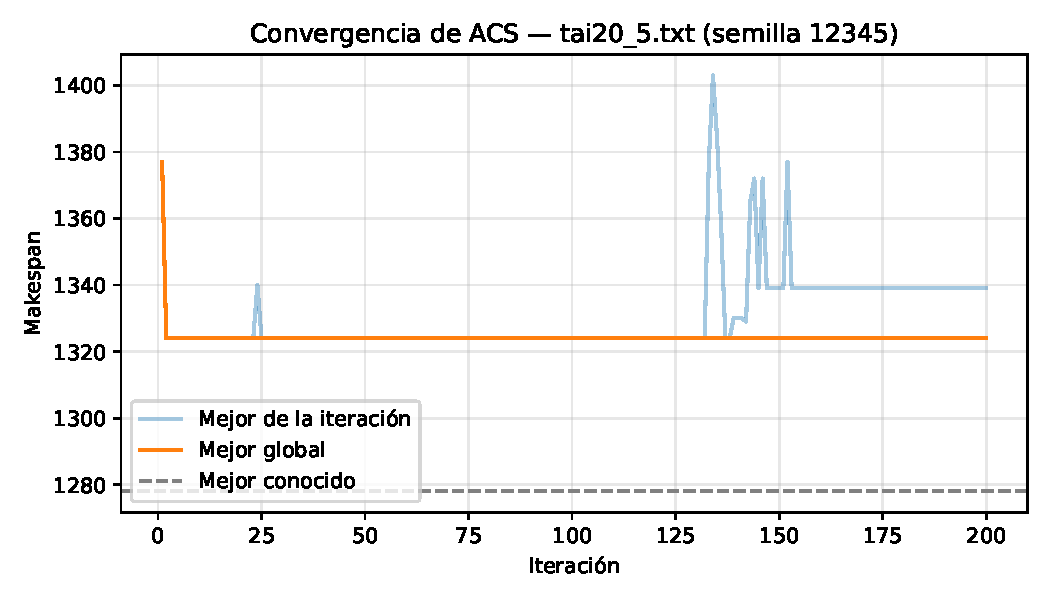
\includegraphics[width=\columnwidth]{../ejercicio_proyecto/graficos/convergencia_tai20_5.pdf}
\caption{Convergencia promedio para la instancia $20\times5$.}
\label{fig:conv20}
\end{figure}

\begin{figure}[t]
\centering
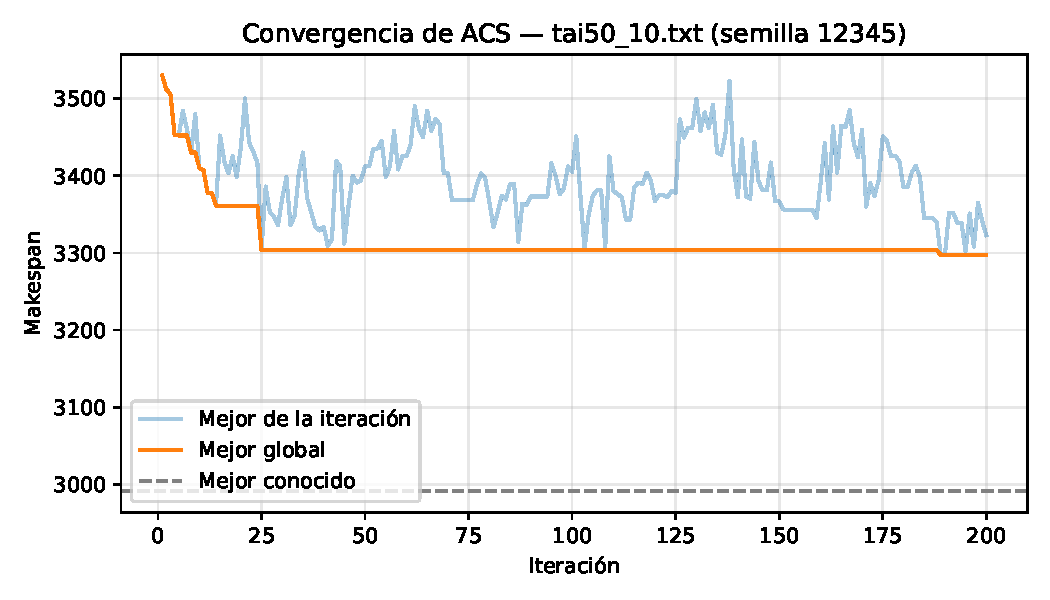
\includegraphics[width=\columnwidth]{../ejercicio_proyecto/graficos/convergencia_tai50_10.pdf}
\caption{Convergencia promedio para la instancia $50\times10$.}
\label{fig:conv50}
\end{figure}

\begin{figure}[t]
\centering
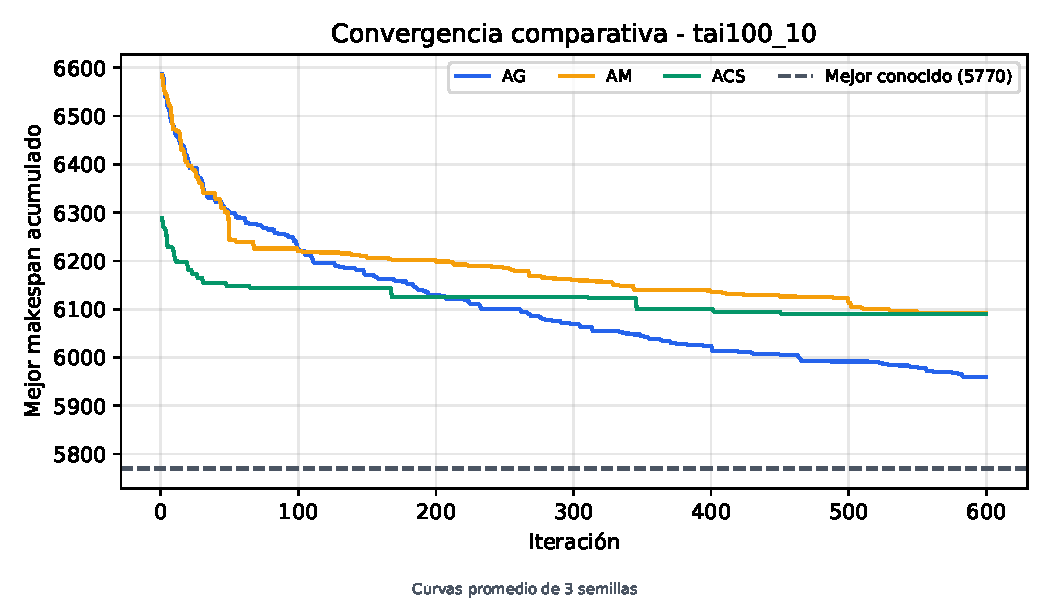
\includegraphics[width=\columnwidth]{../ejercicio_proyecto/graficos/convergencia_tai100_10.pdf}
\caption{Convergencia promedio para la instancia $100\times10$.}
\label{fig:conv100}
\end{figure}

En $20\times5$, las curvas promedio de AG y AM terminan muy próximas. Aunque una ejecución del AM alcanzó 1278 en la iteración 561, la curva no toca la referencia porque representa el promedio de las tres semillas. Para $50\times10$, AM termina con el menor promedio, pero sus resultados individuales muestran mayor sensibilidad a la semilla. AG converge hacia una calidad ligeramente inferior con resultados más estables. ACS mejora durante la ejecución, pero termina por encima de ambos métodos evolutivos.

En $100\times10$, AG continúa mejorando durante gran parte de las 600 generaciones y termina claramente por debajo de AM y ACS. AM también registra mejoras tardías, pero su búsqueda local no cierra la diferencia. ACS se estabiliza antes en una región de peor calidad, lo que sugiere una intensificación prematura de las transiciones reforzadas por feromona.

\subsection{Exploración, explotación y escalabilidad}

AG utiliza cruce y mutación para generar nuevas secuencias, mientras que el elitismo conserva la mejor solución. AM agrega una búsqueda local que prueba mover trabajos dentro de una secuencia para mejorarla. En los experimentos, la configuración de AG obtuvo el mejor resultado promedio y el menor tiempo de CPU en la instancia grande. La de AM alcanzó la referencia en una ejecución pequeña y obtuvo el mejor promedio en la mediana, donde también mostró mayor variación entre semillas y mayor CPU que AG. Estas diferencias corresponden a las configuraciones completas; para medir el aporte de la búsqueda local por separado habría que mantener iguales los demás parámetros.

ACS equilibra exploración y explotación mediante $q_0$, la información heurística y las actualizaciones de feromona. Sin embargo, su visibilidad estática solo aproxima la conveniencia de colocar un trabajo después de otro y no considera el estado completo del prefijo. Esta limitación puede contribuir al estancamiento observado. Además, la construcción secuencial de cada permutación produjo un costo de CPU superior.

Los resultados no identifican un ganador universal. AM fue competitivo en las instancias pequeña y mediana, mientras que AG mostró el mejor desempeño en la instancia grande. ACS no superó a los algoritmos evolutivos con la configuración evaluada. Estas observaciones corresponden exclusivamente a las tres instancias, configuraciones y semillas utilizadas.

\section{Conclusiones y trabajo futuro}

Este trabajo implementó y comparó AG, AM y ACS para minimizar el makespan en el PFSP. Los tres algoritmos utilizaron una representación común, el mismo evaluador y semillas explícitas, lo que permitió realizar una comparación reproducible.

AM obtuvo el menor makespan promedio en $20\times5$ y $50\times10$. En la instancia pequeña, una ejecución alcanzó el valor de referencia de 1278. No obstante, las diferencias promedio entre AG y AM fueron reducidas y AM presentó mayor variación en la instancia mediana. En $100\times10$, la configuración de AG consiguió el menor RPD y el menor tiempo de CPU entre las evaluadas.

ACS obtuvo tiempos de ejecución mayores y no superó a los métodos evolutivos en las instancias estudiadas. Su comportamiento sugiere que la información heurística estática y la actualización de feromona empleadas no fueron suficientes para mantener una exploración efectiva.

El estudio está limitado a una instancia por tamaño, tres semillas y configuraciones ajustadas mediante pruebas preliminares. Por ello, los resultados deben interpretarse de manera descriptiva y no como evidencia de superioridad general de una familia de algoritmos.

Como trabajo futuro se propone aumentar el número de instancias y semillas, comparar los métodos mediante un presupuesto común de tiempo o evaluaciones e incorporar una inicialización basada en NEH. También sería conveniente estudiar una búsqueda local incremental para AM y una visibilidad de ACS dependiente del prefijo construido, con el objetivo de reducir el costo de evaluación y evitar el estancamiento prematuro.

\IEEEtriggeratref{4}
\begin{thebibliography}{9}
\bibitem{Taillard1993}
E.~Taillard, ``Benchmarks for basic scheduling problems,'' \emph{European Journal of Operational Research}, vol.~64, no.~2, pp.~278--285, 1993, doi: \url{https://doi.org/10.1016/0377-2217(93)90182-M}.
\bibitem{Nawaz1983}
M.~Nawaz, E.~E.~Enscore, Jr., and I.~Ham, ``A heuristic algorithm for the $m$-machine, $n$-job flow-shop sequencing problem,'' \emph{Omega}, vol.~11, no.~1, pp.~91--95, 1983, doi: \url{https://doi.org/10.1016/0305-0483(83)90088-9}.
\bibitem{Reeves1995}
C.~R.~Reeves, ``A genetic algorithm for flowshop sequencing,'' \emph{Computers \& Operations Research}, vol.~22, no.~1, pp.~5--13, 1995, doi: \url{https://doi.org/10.1016/0305-0548(93)E0014-K}.
\bibitem{Krasnogor2005}
N.~Krasnogor and J.~Smith, ``A tutorial for competent memetic algorithms: Model, taxonomy, and design issues,'' \emph{IEEE Transactions on Evolutionary Computation}, vol.~9, no.~5, pp.~474--488, 2005, doi: \url{https://doi.org/10.1109/TEVC.2005.850260}.
\bibitem{Dorigo1997}
M.~Dorigo and L.~M.~Gambardella, ``Ant colony system: A cooperative learning approach to the traveling salesman problem,'' \emph{IEEE Transactions on Evolutionary Computation}, vol.~1, no.~1, pp.~53--66, 1997, doi: \url{https://doi.org/10.1109/4235.585892}.
\bibitem{Gmys2021}
J.~Gmys, ``Permutation Flow-shop: Best-known makespans and schedules for Taillard and VFR benchmarks,'' Zenodo, versión 2021, doi: \url{https://doi.org/10.5281/zenodo.4542886}.
\end{thebibliography}
\end{document}
